\section{Experiências e resultados}

\subsection{Análise Dimensional}
Após chegar à ideia base deste problema de o traduzir num sistema de equações, facilmente se pode aumentar a dimensão do problema, que, em termos visuais, é o acréscimo de uma ponta à estrela e, em termos do sistema de equações, é o acréscimo de uma equação. A adição desta nova equação exige, por sua vez, a adição de uma nova restrição.

Para responder à análise dimensional para além das restrições fixas encontradas, que são o caso do sistema de equações caso seja uma estrela de 3 pontas, que é a dimensão mais pequena possível, são também impostas restrições que variam com o tamanho da estrela, podendo desde já se concluir que o número de restrições aumenta linearmente com a dimensão.

De modo a implementar estas restrições foram criados os predicados fixed\_restrictions/3 e growing\_restrictions/3, em que o primeiro aplica as mesmas restrições em qualquer caso e o segundo lida com este aumento de uma equação por ponta adicionada.

\begin{figure}[!htb]
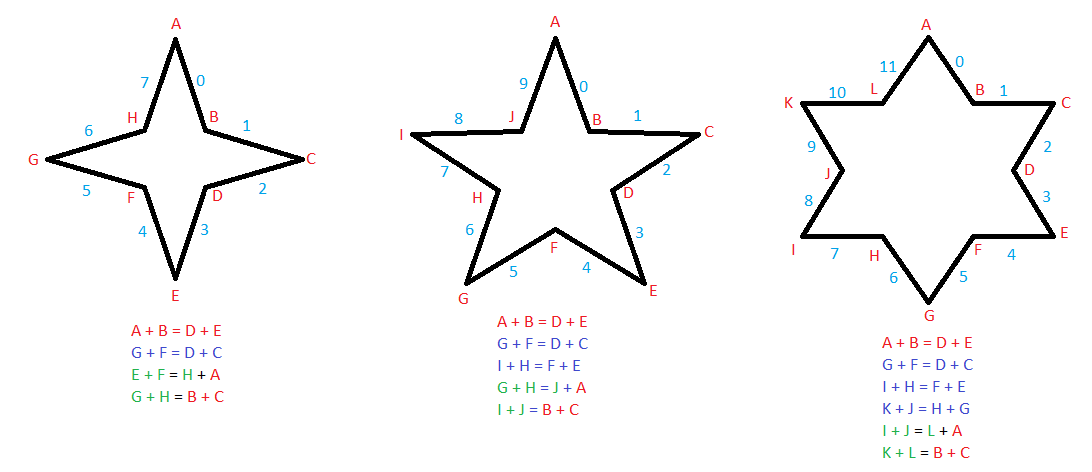
\includegraphics[width=\textwidth]{images/star_analysis.png}
\caption{Esquema descritivo da implementação de restrições} \label{fig:descricao_restricoes}
\end{figure}

Na Figura \ref{fig:descricao_restricoes}, tendo em atenção que as letras representam os operandos e os números os operadores, é possível perceber quais são as restrições fixas e quais as que variam com a dimensão da estrela. As restrições fixas encontram-se a vermelho, a verde estão as restrições que são fixas com o aumento do tamanho, ou seja, são letras que se encontram sempre no mesmo índice relativo na lista de operandos, e a azul as restrições que são acrescentadas com o acréscimo de uma ponta, sendo também visível que se tornam fixas na dimensão acima. Foi com esta análise que foi implementado o predicado growing\_restrictions/3.

% Table generated by Excel2LaTeX from sheet 'Folha1'
\begin{table}[htbp]
  \centering
  \caption{Tempo de execução e número de soluções obtidas com diferentes dimensões}
    \begin{tabular}{lrr}\hline
    \textbf{N º de pontas} & \multicolumn{1}{l}{\textbf{Tempo de Execução(ms)}} & \multicolumn{1}{l}{\textbf{Número de soluções obtidas}} \\ \hline
    \textbf{3 unrestricted} & 563   & 264 \\
    \textbf{3 restricted} & 136   & 132 \\
    \textbf{4 unrestricted} & 15846 & 738 \\
    \textbf{4 restricted} & 3424  & 186 \\
    \textbf{5 unrestricted} & 558125 & 5071 \\
    \textbf{5 restricted} & 80254 & 838 \\
    \textbf{6 unrestricted } & 23416725 & 66334 \\
    \textbf{6 restricted} & 2270679 & 15703 \\ \hline
    \end{tabular}%
  \label{tab:tabela_all_solutions}%
\end{table}%


Na Figura \ref{fig:tempo_execucao_todas_solucoes} e na tabela \ref{tab:tabela_all_solutions} é possível verificar que o aumento do tempo de execução é exponencial com o aumento do número de pontas, assim como o número de soluções, visível na figura \ref{fig:numero_solucoes_todas_solucoes} Por esta razão não foram efetuados teste de dimensão superior a 6 pontas.

\subsection{Estratégias de pesquisa}

A eficiência de um programa em lógica com restrições depende tanto de algoritmos de propagação adequados como de heurísticas apropriadas de seleção da próxima variável a instanciar no processo de enumeração e do valor a atribuir a essa variável.

Foram realizados alguns testes com diferentes combinações heurísticas de ordenação de variáveis, seleção de valores e ordenação de valores para a procura da mesma solução: estrela de 5 pontas com restrições.

Os testes abrangeram todas as combinações possíveis de argumentos de labeling, tanto na parte dos operadores como dos operandos. Os resultados obtidos encontram-se nas tabelas  \ref{tab: heuristicas_operadores} e \ref{tab: heuristicas_operandos}  e nos gráficos \ref{fig:tempo_execucao_combinacoes_heuristicas_operadores} e \ref{fig:tempo_execucao_combinacoes_heuristicas}, respetivamente.
%mudar isto

 Nos resultados obtidos para os operandos, observa-se que a configuração de heurísticas que torna a procura mais eficiente é [min, median, up], aproximadamente 33 segundos mais rápido que a configuração predefinida que é [leftmost,step,up], que melhorou o tempo de execução em 42.5\%; conclui-se também que as configurações consideravelmente menos eficientes são as que usam a heurística occurrence e ffc na ordenação de variáveis,  sendo a configuração menos efieciente [occurence, middle, down], tendo demorado cerca de 4 minutos, o que piora o tempo de execução em 68,4\%. Nestes resultados, é notável a diferença entre o uso de diferentes configurações no labeling.
 
 
 Para os operadores, não se verifica grandes diferenças entre o uso de diferentes configurações no labeling. É possível concluir que a configuração [leftmost,enum,up] é a que torna a procura mais eficiente, tendo melhorado o tempo de execução em 12,7\% e que a configuração [min, bisect,up] é a que torna a procura menos eficiente, tendo piorado o tempo de execução em 65,1\%.
 
 
